%------------------------------------------------------------------------
%  交通流のシミュレーション 
%  The Mathematical Society of Traffic Flow
%  
%  Ver. 1.0 05/12/09  H. Watanabe
%------------------------------------------------------------------------

\documentclass[twocolumn]{jarticle} %二段組の場合
%\documentclass[onecolumn]{jarticle}  %一段組の場合

\usepackage{mstf2}
\usepackage[dvipdfmx]{graphicx}
\usepackage{graphicx}
\usepackage{mathtools}
\graphicspath{{./pic/}}
\usepackage{gensymb}
%------------------------------------------------------------------------

%------------------------------------------------------------------------
%コンパイルコマンド
%1. platex thesis.tex
%2. platex thesis.tex
%3. dvipdfmx thesis.dvi
%4. evince thesis.pdf &
%------------------------------------------------------------------------


\title{%和文タイトル
非線形感覚運動写像ロボットの不完全対面流\\
{\Large -1方向走行流への転移と流量のコース幅依存性-}
}

\titleE{%英文タイトル
Incomplete robots counter flow based on Non-linear sensory motor mapping\\
{\Large -Transition to one-way flow and relations between course and flow rate-}
}

\author{%和文氏名
李 方正$^1$, 橋爪 晋平$^2$,本田 泰$^3$
}

\authorE{%英文氏名
Li Fangzheng$^1$, Shimpei Hashizume $^2$,Yasushi Honda $^3$
}

\affiliation{%和文所属
$^1$ 室蘭工業大学大学院 工学研究科 情報電子工学系専攻\\
$^2$ 室蘭工業大学 工学部 情報電子工学系学科\\
$^3$ 室蘭工業大学大学院 しくみ解明系領域
}

\affiliationE{%英文所属
$^1$ Division of Information and Electronic 
Engineering, Graduate School of Engineering, Muroran Institute of Technology, Japan\\
$^2$ Department Information and Electronic 
Engineering,  School of Engineering, Muroran Institute of Technology, Japan\\
$^3$ College of Information and Systems, Muroran Institute of Technology, Japan
}

\abst{%和文概要
昆虫の群れ行動や混雑した状況での人間の歩行など,
自己駆動粒子の対面流(Counter flow)は広く存在する現象である.
そこでは,レーン形成など自己組織化的な興味深い現象が観察される.

本研究では,われわれは非線形関数(双曲線関数)による感覚運動写像ロボットを開発し,
障害物回避可能な自己駆動粒子とみなす.
そのロボットを使って,擬楕円コースでいくつかのコース幅の対面走行実験を行った.
対面流から1方向流への自律的な転移現象が観測された.

ロボットの速度,流量および1方向流になるまでの時間を測定した.

}

\abstE{%英文概要
In this research, in order to unriddle what kinds of intelligence they have in face-to-face moving of insects and humans, we developed wheeled robot which can avoid obstacles based on Raspberry Pi and we use hyperbolic tangent function to transform distance data which got by three laser sensors to of both sides of motors'power output. Then we have done some face-to-face moving experiments with different numbers'robots on ellipical course and we also measured the speed, flow rate and the time spent of robots change to the same direction.As the result,we observed that all robots tended to moving in the same direction(one direction flow)regardless of initial configuration.And we found that the time of become one direction flow increases with the increase of width and the flow rate increases first and decreases from 49.5cm.



}

%------------------------------------------------------------------------
% ここから本文
%------------------------------------------------------------------------

\begin{document}
\maketitle

\section{はじめに}
   実世界で,蜂,アリなどの昆虫が簡単な振舞いや匂いで複雑な群れ行為ができる.大きな交差点で,人の密度が高いでも,皆は会話なくて,ぶつからないようにスムーズに対面走行ができる.その中に一体どんな知能が持っている,どのぐらいの知能が必要だと知りたいので,我々は原生生物レベルの感覚と運動直接関連する感覚運動写像での障害物避ける振舞い,反応行動レベルの知能を持つ走行ロボットの対面走行を始めにその知能を解明するである.本稿では,tanh関数を使い非線形感覚運動写像をモデルとし,ラズパイを基づく障害物を避ける走行ロボットを開発した.その走行ロボット(今回,最大8台使われる)を右回りと左回り(変曲点係数bで制御する)の2つグループを分けて楕円コースでの対面走行を実験して,変曲点の係数(b)と初期配置を変化させ,ロボットの振舞いを調査して,ロボットたちの時速,同じ流れになるまでの時間と流量などロボットの基本的な走行情報を測定し,one direction flow 状態を観測した.

\section{ロボットの構造}
\subsection{ロボットの身体性}
   走行ロボットの正面図と俯瞰図:
\begin{figure}[h]
    \begin{minipage}{0.48\linewidth}
        \centering
        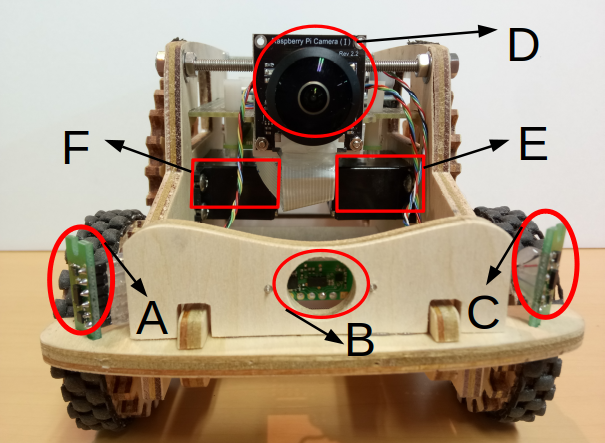
\includegraphics[width=0.9\linewidth]{robot1.jpg}
        \caption{正面図}
    \end{minipage}
    \begin{minipage}{0.48\linewidth}
        \centering
        \includegraphics[width=0.9\linewidth]{robot2.jpg}
        \caption{俯瞰図}
    \end{minipage}
\end{figure}

\begin{figure}[h]
        \centering
        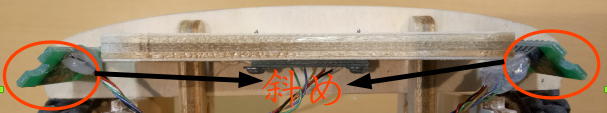
\includegraphics[width=1.0\linewidth]{robot4.jpg}
        \caption{左右のセンサー角度表示}
\end{figure}


A:右の距離センサー;B:中央の距離センサー;C:左の距離センサー;D:カメラ(使っていない);E:右モーター;F:左モーター;制御システム:ラズパイ;左右センサー角度:45\degree;ロボット幅:13.5;ロボット長さ:20.2;ロボット高さ:12.2;



今回使っているのは4輪木造走行ロボットである,人間や昆虫の走行特徴に近似するため,左右の車輪は左右のモーターで独自に制御して,超信地旋回できるようになる.tof距離センサーが赤外線の反射で距離を測るので,超音波より測る範囲が狭いけど,体積が小さく,精度が高くて,複数ロボットの場合,ロボット同士間の妨害も減少できる.


\subsection{ロボット駆動アルゴリズム}
   感覚運動写像とは,センサー値を変数とする関数によってモーターの出力を決定することであり,その瞬間のセンサー値だけを使う,最も単純な反応行動のための知能の一つである.
本研究では,非線形感覚運動写像モデルが使われている.

\subsection{距離データの加重相乗平均}
中央のセンサーによる距離データを $d_{\rm C}$,
また,左のセンサーによる距離データを $d_{\rm L}$ とする.
それらを用いて,左の感覚運動写像の入力 $x_{\rm L}$ を加重相乗平均によって
求める(式(\ref{eq:xL})).
同じように,$d_{\rm C}$と右のセンサーから得られた距離データ $d_{\rm R}$を
用て右の感覚運動写像の入力 $x_{\rm R}$ を求める(式(\ref{eq:xR})).
\begin{eqnarray}
  %x_{\rm L} &=& e^{\gamma \ln d_{\rm C}} \cdot e^{(1-\gamma)\ln d_{\rm L}} 
  x_{\rm L} &=& d_{\rm C}^{\gamma} \times d_{\rm L}^{(1-\gamma)}
  \label{eq:xL} \\
  %x_{\rm R} &=& e^{\gamma \ln d_{\rm C}} \cdot e^{(1-\gamma)\ln d_{\rm R}} 
  x_{\rm R} &=& d_{\rm C}^{\gamma} \times d_{\rm R}^{(1-\gamma)}
  \label{eq:xR}
\end{eqnarray}
$\gamma$は重みであり,本研究においては$\gamma=0.33$とする.
$\gamma=\frac{1}{3}$とすることにより,左のセンサー,中央のセンサーおよび右の
センサーがそれぞれ,$\frac{2}{3}$の等加重となる.

\subsection{感覚運動写像}
\begin{equation}
\begin{aligned}
  m_{\rm R} = &\alpha \tanh(\beta_1(x_{\rm L} - b_{\rm L})) + \\
        &\alpha \tanh(\beta_2(x_{\rm L} - b_{\rm L})) + c
\end{aligned}
\end{equation}

\begin{equation}
\begin{aligned}
  m_{\rm L} = &\alpha \tanh(\beta_1(x_{\rm R} - b_{\rm R})) + \\
        &\alpha \tanh(\beta_2(x_{\rm R} - b_{\rm R})) + c
\end{aligned}
\end{equation}
式(1)と(2)でもらった$x_{\rm L}$と$x_{\rm R}$を式(3)と(4)に代入して,ロボットの右モーターの出力($m_{\rm R}$)と左モーターの出力($m_{\rm L}$)が計算できる.係数$\alpha$がロボットの最大速度を制御する,係数$\beta$が{\rm tanh}の傾きを制御する,係数$b$が関数の変曲点の位置を制御する,係数$c$が関数の縦軸上の位置を制御する. 
今回の実験のパラメーターは
$\alpha$:30.
$\beta_1$:0.004.
$\beta_2$:10.
$c$:0.
ロボットグループ1の$b_{\rm L}$とロボットグループ2の$b_{\rm R}$:160.
ロボットグループ2の$b_{\rm L}$とロボットグループ1の$b_{\rm R}$:260.
   
3.パラメーター$b$の説明:\\
$b_{\rm L}=260$,$b_{\rm R}=160$の場合,$b_{\rm L}=260$のtanh関数の変曲点が$b_{\rm L}=160$のtanh関数の変曲点より横軸の正方向に100移動して(図4の$B$点),$x-b_{\rm L}$が小さくなる,方程式3により,右のモーターが左のモーターより先に速度を減少するので,ロボットが右曲がりやすいである,左曲がり易いのは逆である.
\begin{figure}[!ht]
    \centering
    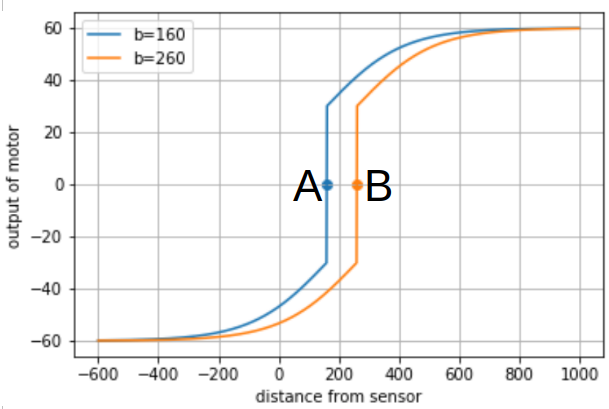
\includegraphics[width=0.7\linewidth]{tanh.jpg}
    \caption{$b=160$と$b=260$のtanh関数の曲線}
\end{figure}


\section{走行実験}
   直線とカーブ両方あり,周期境界条件を持ち複数の対面走行できるように,
楕円コースで実験する.
コースの中(青い部分)にロボットをランダムに配置し,半数のロボットが右回り
($b_{\rm L}>b_{\rm R}$),
残りのロボットが左回り($b_{\rm L}<b_{\rm R}$)の向きで,
速度0からほぼ同時にスタート,約8分間実験する.

ロボットがtof距離センサーでコースの障害物までの距離を測って,
非線形感覚運動写像モデルにより走行する.

コースの青い部分の中央(図\ref{fig:cource}黒い線)でコースの長さを測る,
コースの長さ($L$)は7.32$m$,今回ロボットの台数($N$)は8台.
ロボットの線密度 $ \rho = \frac{N}{L} = 1.09 ({\rm 台/m})$

両側の壁を移動させて,コースの幅($w$)を
$43cm$,$49.5cm$,$56cm$,$62.5cm$,$69cm$へ変化させ,実験する.

\begin{eqnarray}
Q_i &=& \frac{|n_i|}{wT_{\rm sd}}
\label{eq:flow} \\
\bar{Q} &=& \frac{1}{N_{\rm exp}}\sum_{i=1}^{N_{\rm exp}} Q_i
\label{eq:flow_ave} 
\end{eqnarray}

\begin{figure}[h]
    \begin{minipage}{0.48\linewidth}
        \centering
        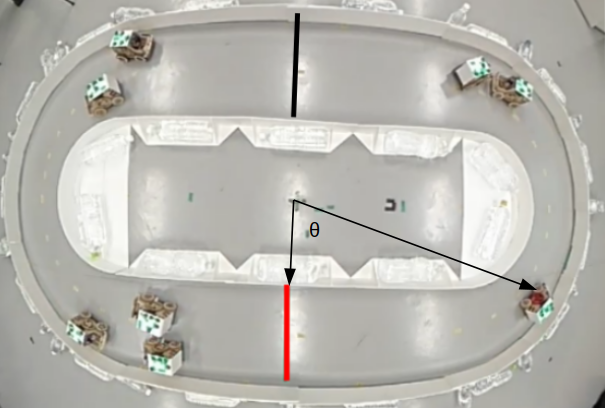
\includegraphics[width=0.9\linewidth]{course3.jpg}
        \caption{コース}
    \end{minipage}
    \begin{minipage}{0.48\linewidth}
        \centering
        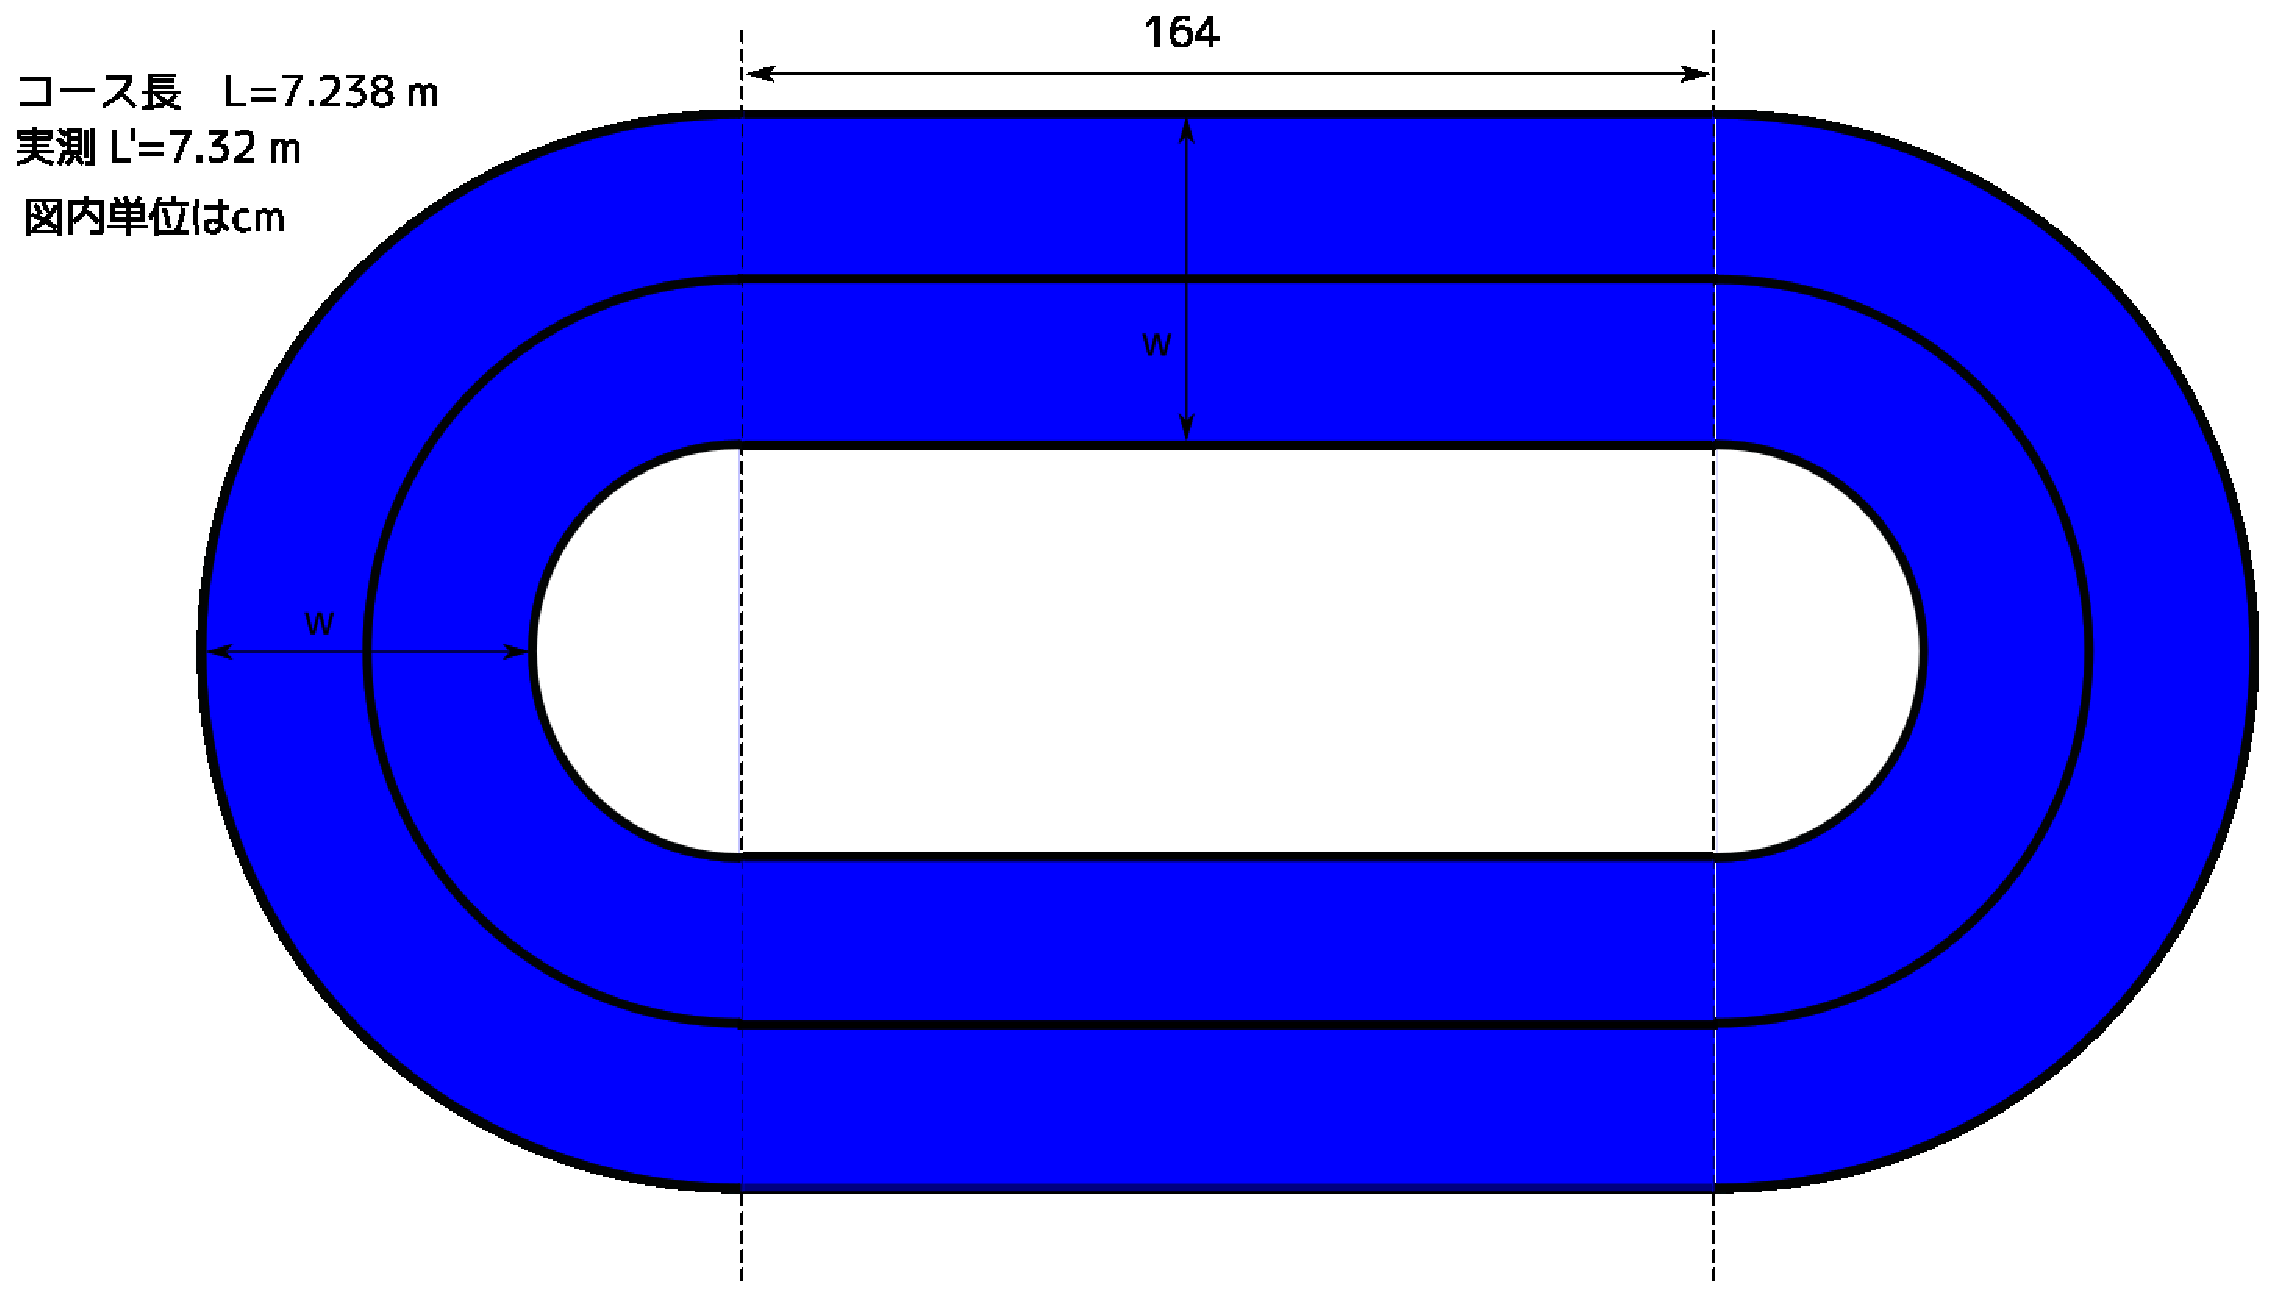
\includegraphics[width=1.0\linewidth]{Oval_h2.eps}
        \caption{\label{fig:cource}コースレイアウト}
    \end{minipage}
\end{figure}



図5の赤い線を計測ラインとして,ロボットが左から右へ線を通過したら流量+1,右から左へ線を通過したら流量-1.図6の横軸が時間(秒),縦軸がコース中心からみたロボットの位置角度$\theta$(図5),ロボットが赤い線から反時計回りで黒い線まで,$\theta$が0から$\pi$に変わる.赤い線から時計回りで黒い線まで,$\theta$が0から$-\pi$に変わる.横軸の時間に従う,$\theta$の変化が$0$を跨ぐと,計測ライン(赤い線)を通過したと認めて,台数($n$)を計測する.$T_{\rm sd}$はone direction flow 状態になる時間(分),$w$がコースの幅(単位:$m$),$Q$が流量,式6で流量を計算する.


\section{実験結果}
\subsection{$T_{\rm sd}$の測定}
  
\vspace{-8mm}
\begin{figure}[!ht]
     \centering
     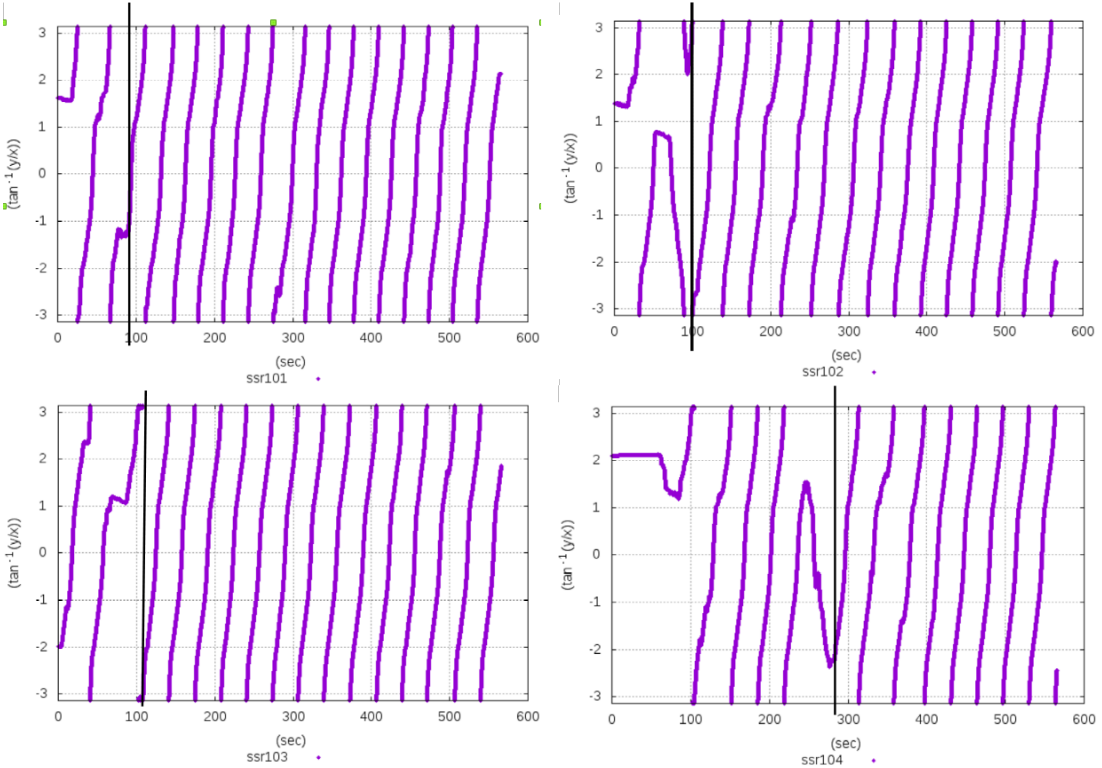
\includegraphics[width=1.0\linewidth]{ssr4_1.jpg}
\end{figure}

\vspace{-8mm}
\begin{figure}[!ht]
     \centering
     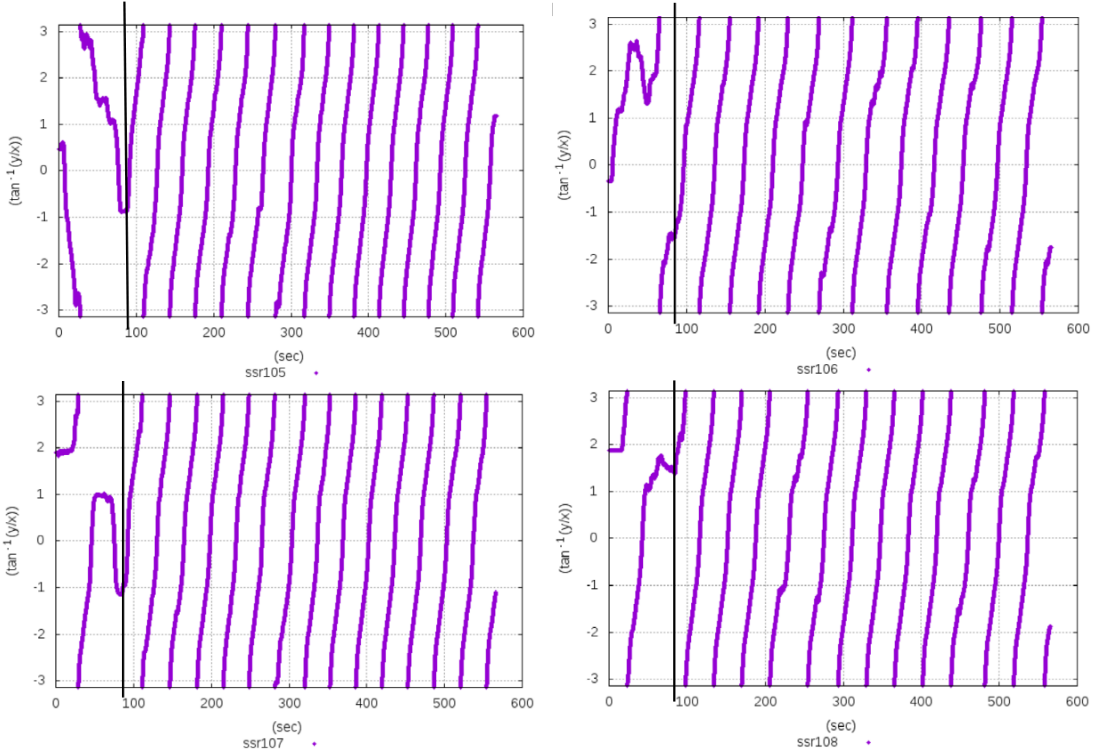
\includegraphics[width=1.0\linewidth]{ssr4_2.jpg}
     \caption{コース中心から見たロボットの角度$\theta$の時間変化}
\end{figure}

図7は各ロボットの$\theta$(図5)と時間の関係図である,横軸は時間(単位:$秒$),縦軸は角度$\theta$である.$T_{\rm sd}$とは全てのロボットが方向転換せず,同じ向きで走る状態になる時間である,図7中の黒い線はロボットが方向転換しなくなるまでの時間,その中で一番長いものを$T_{\rm sd}$とする.





\subsection{初期配置と時速}
   初期配置:ロボットの位置はランダムで,グループ1のロボットが左回りの向き,グループ2のロボットが右回りの向き.

%\item $T_{\rm sd}$:全てのロボットのスタートから全てのロボットが一方向走行するまでの所要時間

各ロボットが一台で5周回って,時速を計算する($v=\frac{5*L}{t}$,$v$:時速,$L$:コースの長さ,$t$:5周回る時間).時速の平均値$\bar v$:13.125$m/min$;標準偏差($s$):51.384


\subsection{幅による$T_{\rm sd}$と流量の測定}
   コースの幅が5つあり,それぞれの幅で十回(毎回8分間)実験する,一実験毎に,ランダムでロボットを2つグループを分ける.$T_{\rm sd}$と流量($Q$)を計測して,平均値と標準偏差を計算する.
\begin{table}[!ht]
\setlength\tabcolsep{1pt}
\begin{center}
\begin{tabular}{|c|c|c|c|c|}
\hline
幅& $\bar{T}_{\rm sd}$ & $s_{T_{\rm sd}}$ & $Q$ & $Q$ \\
($m$)   &  (分) & 標本標準偏差 & 平均値 & 標準偏差 \\
\hline
0.430 & 8.00 & 0 & 0.436 & 0.145 \\
\hline
0.495 & 6.57 & 137.346 & 3.216 & 2.814 \\
\hline
0.560 & 4.63 & 133.561 & 5.248 & 3.394 \\
\hline
0.625 & 4.57 & 106.722 & 3.29 & 2.774 \\
\hline
0.690 & 4.56 & 139.082 & 5.413 & 3.501 \\
\hline
\end{tabular}
\end{center}
\caption{
幅により$T_{\rm sd}$と流量の値
}
\end{table}
\vspace{-6mm}
\begin{figure}[!ht]
    \centering
    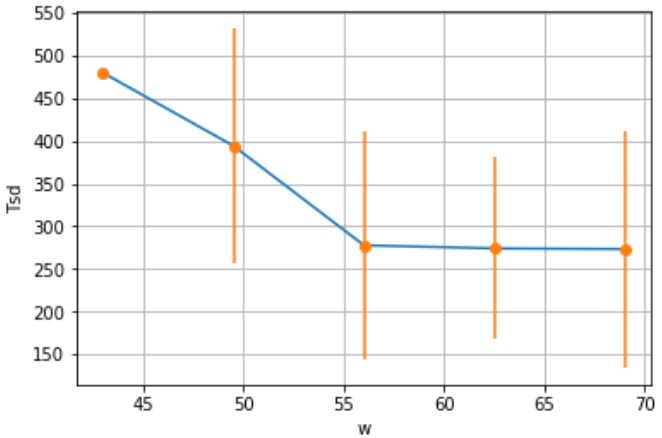
\includegraphics[width=0.8\linewidth]{diagram3.jpg}
    \caption{コース幅 $w$ と$T_{\rm sd}$の関係}
\end{figure}
\vspace{-6mm}
\begin{figure}[!ht]
    \centering
    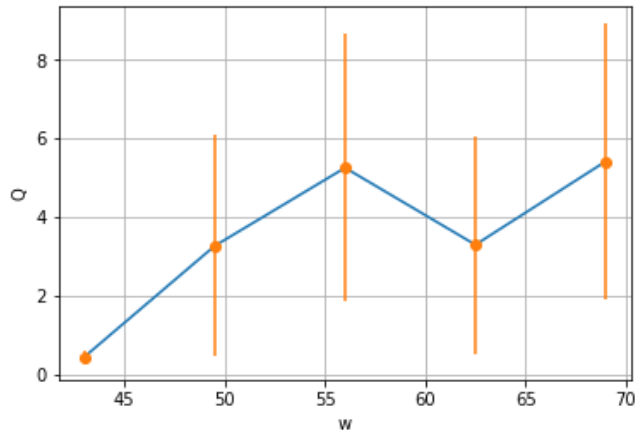
\includegraphics[width=0.8\linewidth]{diagram4.jpg}
    \caption{$Q$とコース幅の関係}
\end{figure}

図$8$はコース幅($w$)による,$T_{\rm sd}$平均値の変化曲線である.図$9$がコース幅による,平均流量($Q$)の変化曲線である.幅が狭すぎる(43$cm$)と,長時間の渋滞が発生したことを観測した,ロボット同士のすれ違い,方向転換ができず,one direction flow の状態とならなかった.大渋滞なので,流量もほとんどない.49.5$cm$の場合,渋滞が発生したので,one direction flow 状態になる時間($T_{\rm sd}$)も長かったが,ロボットが方向転換できたので,流量も多少増えた.56$cm$から渋滞の発生が急激に減少し,ロボットの方向転換もしやすくなり,$T_{\rm sd}$が減少した.以降コース幅が拡大しても,$T_{\rm sd}$に明らかな変化が見られなくなった.56$cm$まで平均流量が増えて,$62.5cm$の場合,平均流量が多少減少したと観測した.


\section{まとめ}
   \input{summary3c}

\begin{thebibliography}{99}
\bibitem{asada} 浅田稔,国吉康夫.「ロボットインテリジンス」P1-59,(2006).
\bibitem{yamada} 山田将司,大園章宏,本田泰.2次元最適速度ロボットの多様な集団紐状走行.第25回交通流と自己駆動粒子系シンポジウム論文集.(2019)
\bibitem{ikeda} 池田光佑,金鋼.対向する自己駆動粒子系におけるレーン形成とその動的な転移の解明.(2016)
\bibitem{ishi} 石渡龍輔,衣川亮太,杉山雄規.Kantorovich metricを用いた2次元OV粒子の集団流の感応度依存性の解析.(2016)
\bibitem{kawano} 川野多佳也,宮島高志,本田泰.二次元最適速度ロボットの開発と集団走行実験.(2017)
\end{thebibliography}
\end{document}

\end{document}




